\documentclass[10pt]{article} % For LaTeX2e
\usepackage{tmlr}
% If accepted, instead use the following line for the camera-ready submission:
%\usepackage[accepted]{tmlr}
% To de-anonymize for a preprint server, instead use:
%\usepackage[preprint]{tmlr}

\usepackage{amsmath, amssymb, amsfonts, amsthm}
\usepackage{graphicx}
\usepackage{booktabs}
\usepackage{multirow}
\usepackage{hyperref}
\usepackage{url}

\newtheorem{proposition}{Proposition}

% Values quoted inside captions, generated from the artifacts.
\newcommand{\PrescoreK}{2}
\newcommand{\SPBfFourHi}{2.71}
\newcommand{\SPBfFourLo}{1.76}
\newcommand{\SPBfOneHi}{1.06}
\newcommand{\SPBfOneLo}{0.85}
\newcommand{\SPBfTwoHi}{1.66}
\newcommand{\SPBfTwoLo}{1.10}
\newcommand{\SPTfOneHi}{0.82}
\newcommand{\SPTfOneLo}{0.62}
\newcommand{\SPTfTwoHi}{1.01}
\newcommand{\SPTfTwoLo}{0.78}
\newcommand{\SelectorsK}{4}
\newcommand{\SmallNComposedHi}{9.8}
\newcommand{\SmallNComposedLo}{2.7}
\newcommand{\SmallNHostFixed}{61}
\newcommand{\SmallNPerLaunch}{9}
\newcommand{\SmallNRhoFlops}{0.03}
\newcommand{\SmallNRhoLaunch}{0.95}
\newcommand{\SmallNZorderHi}{22}
\newcommand{\SmallNZorderLo}{8}
\newcommand{\StagesCaption}{Peak measured on the same device: 57.8~TFLOP/s and 1497~GB/s, a ridge point of 39~FLOP/byte.}
\newcommand{\StagesN}{512}
\newcommand{\StreamFindHi}{91}
\newcommand{\StreamFindLo}{85}
\newcommand{\StreamKFourDev}{15}
\newcommand{\StreamKFourHi}{1.15}
\newcommand{\StreamKFourLo}{0.91}
\newcommand{\StreamKOneLo}{0.50}
\newcommand{\StreamKTwoHi}{0.84}
\newcommand{\StreamRowsM}{34}


\title{The FLOPs You Save Are Not the Time You Spend:\\
Sparse Attention in Multi-Agent Communication}

% Authors must not appear in the submitted version. They are hidden as long as
% the tmlr package is used without the [accepted] or [preprint] options.
\author{\name Anonymous \email anonymous@example.com \\
      \addr Anonymous Institution}

\def\month{08}  % Insert correct month for camera-ready version
\def\year{2026} % Insert correct year for camera-ready version
\def\openreview{\url{https://openreview.net/forum?id=XXXX}} % Insert correct link

\begin{document}

\maketitle

\begin{abstract}
Sparse attention in multi-agent communication is usually justified by the
operations it removes. We charge each peer-selection rule for what deciding
costs, and measure on four GPUs, from A100 to Blackwell, when the saving becomes
elapsed time.
First, a rule that ranks attention scores must compute all of them, so it
removes at most half of the forward-pass multiply--accumulates at any sparsity;
rules that select before scoring escape this ceiling by as much as their
selector is cheap. Second, composed from library operators, score-then-select
attention is slower than dense attention at every configuration we measure, by
up to 37 times, because compacting the retained peers adds more memory traffic
than it removes. A fused kernel that streams the selection is faster than dense
attention with one or two retained peers in fp32 and, up to 512 agents, within
15\% of parity with four and slower with eight; and from 384 agents upward at least 85\% of its time is spent
finding the retained set; in bf16 only one retained peer breaks even. On A100,
H100 and H200 the streaming kernel wins everywhere only with one retained peer,
and in bf16 not at all. Third,
once the set is known without scoring, attention over it is up to 16 times
faster than dense attention, and the selector decides the outcome: of three
selectors, only the cheapest reaches parity, at 512 agents, on best-case
timings and on the Blackwell card only. Below 100 agents, where multi-agent methods are usually evaluated, the
number of kernels a step launches orders latency, and its operation count does
not.

\end{abstract}

\section{Introduction}
\label{sec:intro}
Cooperative multi-agent systems increasingly exchange learned messages, and
attention is a common way of deciding whose message matters
\citep{das2019tarmac,jiang2018atoc,jiang2018dgn}.\footnote{\LLMDisclosure}
Attention over $N$ agents is pairwise, so its cost grows quadratically, and
several methods restrict who attends to whom, citing communication or
computational cost among their reasons
\citep{jiang2018dgn,sun2020sparsecomm}. The computational
argument is an operation count: if each agent aggregates messages from $k$ peers
instead of $N-1$, the aggregation shrinks by a factor of about $N/k$.

This paper asks when that saving becomes elapsed time. Three costs have to be
separated, and an operation count conflates them. The first is \emph{what can
be removed at all}: a rule that selects peers by their attention scores needs
the scores, so every pairwise score has been computed by the time the selection
is made, and only the aggregation can shrink. The second is \emph{what the
implementation executes}: masking the discarded weights to zero leaves the
dense multiplication in place, while gathering the retained values removes it
and writes new intermediates instead. The third is \emph{what the hardware
spends its time on}: at the agent counts and head widths of this setting,
attention is memory-bound, so an implementation that removes arithmetic while
adding data movement can become slower. We study centralised inference on a
single device, the setting in which the methods we cite are trained and
evaluated, and not bandwidth-constrained distributed deployment, where reducing
transmitted messages is itself the objective.

\paragraph{Findings.} For \emph{score-then-select} rules, which form every score
before keeping the $k$ largest, at most half of the forward-pass attention
multiply--accumulates are removable at any sparsity, a limit noted before in a
memory-access model \citep{chen2023dfss}. Composed from library operators, such a rule is slower than dense attention at every agent count and sparsity we measure, the gathered form by up to thirty-seven times, because of memory traffic. A fused kernel
is faster than the best dense implementation only when one peer is retained (two
at a single configuration), at head widths $16$ and $32$, and without tensor
cores; in TF32 and bf16 the advantage is gone from $384$ agents upward. One
retained peer is a degenerate attention, since a softmax over one element is
identically one. Handing the fused kernel's own retained set to a kernel for free
shows where its time goes: from $384$ agents upward, at least nine tenths is
spent finding the set. Rules that \emph{select before scoring} escape the bound,
and attention over a pre-selected set is then up to sixteen times faster than
dense attention, but the selector decides the outcome: of an all-pairs, a grid
and a space-filling-curve selector, only the last reaches parity with dense
attention, at $512$ agents on best-case timings, and the ratio of medians
reverses that in one of our two sweeps.

\paragraph{Contributions.}
\begin{itemize}
  \item A cost model for peer selection (Section~\ref{sec:analysis}): a
    closed-form multiply--accumulate limit on score-then-select for the forward
    and backward passes (Proposition~\ref{prop:ceiling}); a selector-cost
    accounting that sorts selection mechanisms into four asymptotic classes
    (Proposition~\ref{prop:escape}, Corollary~\ref{cor:taxonomy}); and a byte
    criterion, $kd \le N$, that screens compaction before implementation.
  \item A measurement of what is executed (Section~\ref{sec:measurement}):
    masked, gathered and fused implementations of one function, verified
    equivalent, against the best of a vendor library, FlexAttention and a dense
    kernel searched over the sparse kernels' parameter space; three numerical
    formats; and a fixed-set comparison that separates the cost of finding the
    retained peers from the cost of using them.
  \item A characterisation of when sparse attention is faster in this regime:
    narrowly for score-then-select, and more broadly for selection before
    scoring when the selector is cheap in absolute terms and the remaining
    attention is fused (Sections~\ref{sec:fused}--\ref{sec:prescore}).
\end{itemize}

We release the kernels, the harness and the scripts that regenerate every table
and figure and check the quoted numbers. A pre-registered training study
(Appendix~\ref{app:training}) shows that the communicating architecture improves
return under the evaluated setup; it is not powered to rank sparsification
variants, and no claim in the main text rests on it. The measured envelope is
one GPU architecture, head widths $16$ to $512$ and at most $512$ agents
(Section~\ref{sec:limitations}).


\section{Related Work}
\label{sec:related}
\paragraph{Communication sparsity in multi-agent reinforcement learning.}
Learned inter-agent communication has converged on attention for deciding whose
message matters: CommNet broadcasts mean-pooled hidden states
\citep{sukhbaatar2016commnet}, TarMAC introduces signature-based targeting
\citep{das2019tarmac}, and MAT casts the joint policy as a sequence model
\citep{wen2022mat}. Because attention over $N$ agents is pairwise, much of this
literature restricts who communicates, usually motivated by cost; DGN observes
that receiving much information ``requires high bandwidth and incurs high
computational complexity'' \citep{jiang2018dgn}. Corollary~\ref{cor:taxonomy}
sorts these mechanisms by what their selector costs. DGN's nearest neighbours,
ATOC's communication field and mean-field interaction fix the retained set from
structure available before any score exists
\citep{jiang2018dgn,jiang2018atoc,yang2018meanfield}; they are free if the
neighbourhood arrives with the environment and case~(b) if it is recomputed from
all pairwise positions each step. IC3Net and SchedNet gate or rank agents by a
scalar per agent, a top-$k$ over an $O(N)$ vector rather than an $N \times N$
matrix \citep{singh2018ic3net,kim2019schednet}. G2ANet and MAGIC run a pairwise
hard-attention or graph-construction network before communication attention
\citep{liu2020g2anet,niu2021magic}, so their selector is of the same order as
the scores they avoid. Score-then-select is the limiting case: the adaptive
sparse communication graph of \citet{sun2020sparsecomm} applies a sparsemax
generalisation to logits already formed for every pair and motivates it partly
by reduced complexity, and handshake mechanisms that match a query against every
candidate key before selecting \citep{liu2020who2com} are score-then-select in
the same sense. These methods operate with two to roughly thirty agents, DGN reaching the low
hundreds. Of the multi-agent papers we relied on that make an efficiency claim,
one of five reports a measured time attributable to the mechanism
(Appendix~\ref{app:audit}).

\paragraph{Efficient and sparse attention.} Efficient-attention methods
separate along the same axis. Sparse Transformers, Longformer and BigBird fix
the interaction pattern in advance, so the score computation itself is sparse
and the selector is essentially free
\citep{child2019sparse,beltagy2020longformer,zaheer2020bigbird}. Reformer and
Routing Transformer restrict candidates by hashing and online clustering, which
are content-dependent but evaluate scores only for candidate pairs, at a
selector cost that must be counted \citep{kitaev2020reformer,roy2021routing}.
Performer keeps every interaction and reorders the algebra
\citep{choromanski2021performers}. Top-$k$ attention in sequence models is the
closest analogue of our mechanism: the Explicit Sparse Transformer keeps the $k$
largest scores per query \citep{zhao2019explicit}, and \citet{gupta2021topk}
compute each query's exact top-$k$ over all keys in chunks, with memory
efficiency as the stated benefit. Sparsemax and $\alpha$-entmax obtain exact
zeros from the normalisation rather than a hard cutoff
\citep{martins2016sparsemax,peters2019entmax}; because their zeros arrive after
the scores exist, they fall under Proposition~\ref{prop:ceiling}, which is our
inference rather than a claim they make. Sparse mixture-of-experts routing is
also score-then-select \citep{shazeer2017moe,fedus2022switch}, but the router is
small relative to the expert computation it gates, so the analogue of our score
term is minor and the saving is real. Whether score-then-select pays therefore
depends on the ratio between the cost of scoring every candidate and the cost
of the work skipped, which is one in single-head attention. 

\paragraph{Hardware-aware execution.} That operation counts do not determine
runtime is established in general terms \citep{dehghani2022misnomer}, and
transformer workloads are known to be dominated by data movement rather than
arithmetic \citep{ivanov2021datamovement}; the roofline model formalises when
arithmetic ceases to govern runtime \citep{williams2009roofline}. FlashAttention
and its successors reduce memory traffic without changing the operation count
\citep{dao2022flashattention,dao2024flashattention2,shah2024flashattention3,rabe2021selfattention},
and FlexAttention compiles attention variants expressed as score modifications
and block masks into fused kernels \citep{dong2025flexattention}. Native Sparse
Attention and MiniMax Sparse Attention show where sparse attention does pay:
blockwise selection amortises the selector over blocks, preserves matrix-multiply
shapes inside selected tiles, and operates at $10^4$ to $10^6$ tokens, where the
skipped work is large \citep{yuan2025nsa,lai2026msa}. Relative to this
literature our contribution is specific: a selector-cost accounting that
separates mechanisms before measurement, a byte criterion for per-pair
compaction, and measurements at tens to hundreds of agents and narrow heads,
where neither block amortisation nor large skipped work is available. Our benchmarking follows
established practice for reporting performance on shared hardware
\citep{hoefler2015benchmarking}, and our kernels are written in Triton
\citep{tillet2019triton}. The training study follows
\citet{papoudakis2021epymarl} and \citet{agarwal2021rliable}, with environments
from PettingZoo/MPE \citep{terry2020pettingzoo} and MAPPO
\citep{yu2022mappo}.


\section{Computational Limits of Score-Then-Select Attention}
\label{sec:analysis}
\subsection{Problem setting}
\label{sec:setting}

Consider one round of scaled dot-product attention over $N$ agents, per batch
element, at head width $d$. Agent $i$ forms a query $q_i$; every agent
contributes a key and a value; self-attention is masked. Write
$s_i = q_i K^\top \in \mathbb{R}^N$ for the score vector and
$a_i = \mathrm{softmax}(s_i)$ for the attention weights, so that dense attention
computes $m_i = a_i V$. A top-$k$ variant keeps the $k$ largest entries of $a_i$
and renormalises over them.

The mechanism this paper analyses is the one that arises most naturally from
that description: form the complete score vector, then keep its $k$ largest
entries. We call such a rule \emph{score-then-select}, and the term is used in
its exact sense throughout. Every analytic claim below concerns that class, not
content-dependent selection in general, and Section~\ref{sec:ceiling} draws the
boundary.

Attention has two matrix products of equal size. One produces the pairwise
scores; the other aggregates the values. Sparsifying the retained set shrinks
the second, because only $k$ value rows are combined. It cannot shrink the
first, because the scores are what the selection reads. That observation is the
whole of Section~\ref{sec:ceiling}; the rest of this section makes it precise
and marks where it stops applying.

Top-$k$ attention admits three implementations of the identical function, and
the distinction between them is what separates an arithmetic saving from an
executed one.

\begin{description}
  \item[Masked top-$k$.] Compute $a_i$ in full, multiply by a $\{0,1\}$ mask,
    renormalise, and evaluate $m_i = \tilde{a}_i V$ with $\tilde{a}_i$ still
    dense in memory. The discarded entries are materialised as zeros and
    multiplied, so the executed aggregation count is unchanged from dense while
    selection, masking and renormalisation are added on top.
  \item[Gathered top-$k$.] Take the top-$k$ of the raw scores, softmax over
    those $k$ values, gather the corresponding value rows into a $(B,N,k,d)$
    tensor, and contract $(B\!\cdot\!N,1,k)\times(B\!\cdot\!N,k,d)$. No zeros
    are materialised and the aggregation genuinely shrinks.
  \item[Fused top-$k$.] Compute the same function in a single kernel, holding
    the score row in registers, selecting within them, and accumulating the
    weighted values without writing a score matrix, an index tensor or a
    gathered value tensor to memory. Section~\ref{sec:fused} reports one.
\end{description}

\begin{figure}[t]
\centering
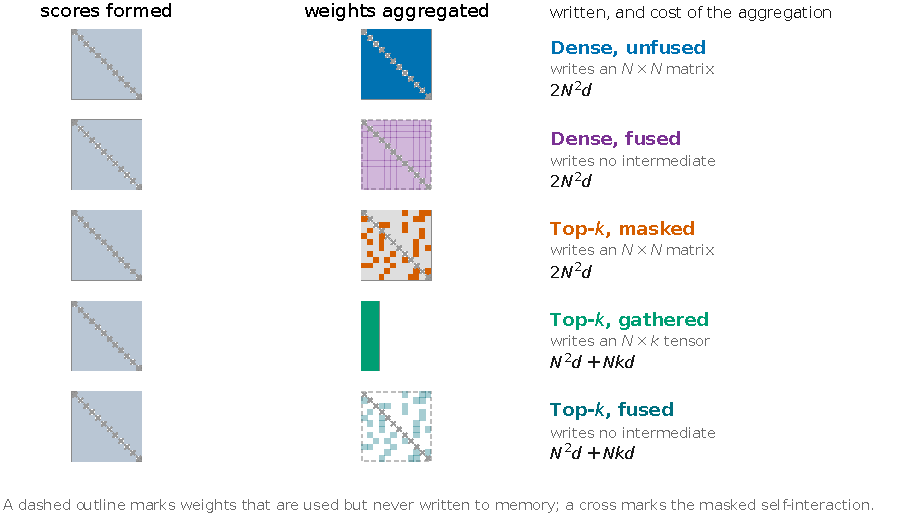
\includegraphics[width=\linewidth]{figures/fig1_taxonomy.pdf}
\caption{Two implementations of dense attention and three of top-$k$ attention,
computing two functions in five ways. All five evaluate every pairwise score,
because a score-then-select rule must form the complete score vector before it
can rank it. They differ in what reaches memory and in how much arithmetic the
aggregation performs, and only the gathered and fused top-$k$ variants execute
the saving that motivates sparsification at all. The fused row stands for the
kernels that compact the retained set; the threshold kernel of
Section~\ref{sec:fused} is fused in the same sense but keeps the dense
aggregation, so its cost is that of the masked row.}
\label{fig:taxonomy}
\end{figure}

Gathered and masked top-$k$ compute the same function
(Figure~\ref{fig:taxonomy}). Softmax is monotone within a row, so the top-$k$
weights are the top-$k$ scores, and a softmax over just those $k$ scores equals
the dense softmax restricted to them and renormalised; the two agree to
$<10^{-10}$ in \texttt{float64} (Appendix~\ref{app:verification}). The
operation-count argument is about the gathered variant. Timing the masked
variant measures an implementation artifact, and timing either against unfused
dense alone ignores what a production kernel costs, so we report all
implementations against both dense baselines throughout.

\subsection{An operation-count ceiling}
\label{sec:ceiling}

Analytic counts are multiply--accumulates. Under the convention that a
multiply--add is two floating-point operations every term doubles and every
ratio is unchanged, so the ceiling is the same number either way; we write MACs
where the count is analytic and FLOPs only where a counter attached to the
running program produced the figure. Counting the two matrix products that
constitute attention, and excluding the shared input and output projections:
\begin{equation}
C_{\text{scores}} = N^2 d, \quad C_{\text{agg}} = N^2 d, \quad
C_{\text{dense}} = 2N^2 d, \qquad
C_{\text{top-}k} = \underbrace{N^2 d}_{\text{all scores}} +
\underbrace{Nkd}_{\text{aggregate }k}.
\end{equation}

\begin{proposition}[Score-then-select ceiling]
\label{prop:ceiling}
Let the retained set be fixed by a score-then-select rule, one whose kept
indices are determined only after the complete score vector of each query has
been formed. Then
\begin{equation}
\frac{C_{\text{dense}}}{C_{\text{top-}k}}
= \frac{2N^2 d}{N^2 d + Nkd} = \frac{2N}{N+k} < 2
\qquad \text{for all } k \ge 1,
\end{equation}
with supremum $2$ approached only as $k/N \to 0$. Within this class, no choice
of $k$ or $N$ yields more than a twofold reduction in attention MACs.
\end{proposition}

\begin{proof}
$C_{\text{top-}k} > N^2 d = \tfrac12 C_{\text{dense}}$ for every $k \ge 1$ since
$Nkd > 0$, so the ratio is below $2$. It is decreasing in $k$, hence largest at
$k = 1$, and approaches $2$ from below as $k/N \to 0$.
\end{proof}

The familiar figure $1 - k/(N-1)$ describes the value-aggregation term alone.
Read as \emph{the} saving it overstates the achievable reduction by a factor
approaching two, before any question of whether the reduction is realised in
time.

We use $N^2 d$ rather than $N(N{-}1)d$ because it is the count the
implementations execute: self-masking writes $-\infty$ into the diagonal of a
full $N \times N$ score matrix and does not skip work. Counting the diagonal
exactly gives $2(N{-}1)/\bigl((N{-}1)+k\bigr)$, which is strictly smaller for
every $1 \le k \le N-1$, so the proposition is a valid upper bound under either
convention.

The ceiling is a statement about the forward pass, and training moves it. Exact
selection is piecewise constant in the scores, so gradients reach only the
retained entries: of the four products in dense attention's backward pass
(the gradients with respect to values, weights, queries and keys, each
$N^2 d$), a gathered top-$k$ backward executes each over the $Nk$ retained pairs
alone, given the indices recorded in the forward pass. Counting both passes,
without recomputation,
\begin{equation}
\frac{C^{\text{f+b}}_{\text{dense}}}{C^{\text{f+b}}_{\text{top-}k}}
= \frac{6N^2 d}{N^2 d + 5Nkd} = \frac{6N}{N+5k} < 6,
\end{equation}
so in training at most five sixths of attention's arithmetic is removable,
against half in inference. The asymmetry is visible in the measurements of
Section~\ref{sec:backward}, where the gathered path's backward is cheap relative
to its forward.

Six assumptions support the statement, of which only the second is essential.
\textbf{(A1) Single round}: with $R$ rounds both terms scale by $R$ and the
ratio is unchanged. \textbf{(A2) Full-score selection}: the retained set is
determined only after the complete candidate score vector has been computed, so
all $N$ scores must be formed. \textbf{(A3) Per head}: with $H$ heads of width
$d/H$ both terms scale identically. \textbf{(A4) Projections excluded}:
including the shared $qkv$ and output projections moves the ratio strictly
closer to $1$, so the bound remains valid. \textbf{(A5) Selection cost
excluded}: counting the top-$k$ operation itself can only decrease the ratio,
and Section~\ref{sec:stages} shows the term is large in practice.
\textbf{(A6) Equal key and value widths}: with key width $d_k$ and value width
$d_v$ the two products cost $N^2 d_k$ and $N^2 d_v$, and the ceiling is
$1 + d_v/d_k$, which is $2$ in the equal-width attention used throughout.

A2 concerns \emph{when} the retained set is fixed, not whether the rule depends
on the data. Mechanisms that are content-dependent but not score-then-select lie
outside the class and are unconstrained by Proposition~\ref{prop:ceiling}: exact
or approximate nearest-neighbour retrieval, clustering and routing, indexing and
hashing can all identify candidates without materialising the complete pairwise
score matrix. Routing Transformer's online $k$-means routing
\citep{roy2021routing} and Reformer's locality-sensitive hash
\citep{kitaev2020reformer} are content-dependent in every ordinary sense and
still evaluate scores only for candidate pairs; a hierarchical rule that ranks
compressed blocks and then scores only the selected ones \citep{yuan2025nsa} is
likewise outside A2. What such rules pay instead is a selector cost, and the
next proposition charges them for it.

\subsection{Selection before scoring}
\label{sec:escape}

\begin{proposition}[Escape]
\label{prop:escape}
Suppose the kept set is determined \emph{without} forming the complete score
vector --- structurally, or by a retrieval, routing, clustering, indexing or
hashing rule --- at total selector cost $C_{\mathrm{sel}}(N,k,d)$, and that
attention scores are then evaluated only for the $Nk$ retained pairs. Then
\begin{equation}
C_{\mathrm{pre}} = 2Nkd + C_{\mathrm{sel}},
\qquad
\frac{C_{\text{dense}}}{C_{\mathrm{pre}}}
  = \frac{2N^2 d}{2Nkd + C_{\mathrm{sel}}}.
\end{equation}
\emph{(i)} If $C_{\mathrm{sel}} = o(Nkd)$ --- in particular for a fixed or
precomputed pattern, where $C_{\mathrm{sel}} \approx 0$; note that an
$O(N \log N)$ selector does \emph{not} qualify, since
$N\log N / (Nkd) = \log N/(kd) \not\to 0$ --- the ratio is
asymptotic to $N/k$, that is
$\bigl(C_{\text{dense}}/C_{\mathrm{pre}}\bigr)\big/(N/k) \to 1$. Exact equality
with $N/k$ holds only when $C_{\mathrm{sel}} = 0$; for every
$C_{\mathrm{sel}} > 0$ the ratio is strictly smaller. \emph{(ii)} If only
$C_{\mathrm{sel}} = o(N^2 d)$ and $k/N \to 0$, the ratio diverges, and in
particular is not bounded by $2$, though it does not in general grow at the
rate $N/k$.
\end{proposition}

\begin{proof}
Both statements read off the displayed ratio. For (i),
$2Nkd + C_{\mathrm{sel}} = 2Nkd\,(1+o(1))$, so
$C_{\text{dense}}/C_{\mathrm{pre}} = (N/k)\,(1+o(1))^{-1}$, whose quotient with
$N/k$ tends to $1$; substituting $C_{\mathrm{sel}} = 0$ gives
$2N^2 d/2Nkd = N/k$ exactly, and any $C_{\mathrm{sel}} > 0$ strictly enlarges
the denominator. For (ii), if $k/N \to 0$ then $2Nkd = o(N^2 d)$, so the whole
denominator is $o(N^2 d)$ and the ratio diverges.
\end{proof}

Proposition~\ref{prop:ceiling} is the limiting case of this accounting. A
score-then-select rule must form the full score matrix before it can rank it,
and in doing so it has already evaluated the scores of the $Nk$ retained pairs,
which the displayed form charges again inside $2Nkd$. Written in that form its
selector cost is therefore at least the scores of the discarded pairs,
$C_{\mathrm{sel}} \ge N^2 d - Nkd$, and this is a lower bound and not an
estimate: the ranking itself is uncounted, and counting it enlarges
$C_{\mathrm{sel}}$ and shrinks the ratio further. Substituting the bound gives
$2N^2d/(N^2d + Nkd)$, which is Proposition~\ref{prop:ceiling}; any real
implementation sits below it. Reading the two propositions as one statement
places any peer-selection mechanism on a single axis, the cost of deciding what
to keep, and the position on that axis determines what the mechanism can save.

\begin{corollary}[What a selector costs, and what it can therefore buy]
\label{cor:taxonomy}
Count $C_{\mathrm{sel}}$ in multiply--accumulate equivalents, one comparison,
integer operation or distance term being one unit. Fix $k$ and $d$ and let
$N \to \infty$ in $S = 2N^2d/(2Nkd + C_{\mathrm{sel}})$.
\emph{(a) Full-score selection}, $C_{\mathrm{sel}} \ge N^2 d - Nkd$: $S < 2$.
\emph{(b) All-pairs selection in a cheaper feature dimension $p \ll d$},
$C_{\mathrm{sel}} = \gamma N^2 p$: $S \to 2d/(\gamma p)$, a constant that does
not grow with $N$ and does not improve with $k$.
\emph{(c) Sub-quadratic selection}, $C_{\mathrm{sel}} = \Theta(N \log N)$:
$S = \Theta\bigl(Nd/\log N\bigr)$, which diverges, but is a vanishing fraction
of $N/k$.
\emph{(d) Fixed or precomputed patterns}, $C_{\mathrm{sel}} = o(Nkd)$ and in
particular $C_{\mathrm{sel}} \approx 0$: $S \sim N/k$. A selector with
$C_{\mathrm{sel}} = cNkd$ for a constant $c > 0$ gives $S \to 2N/((2+c)k)$,
which is $\Theta(N/k)$ but not asymptotic to it.
\end{corollary}

The asymptotic classes do not depend on the unit convention; the constants in
the closed forms below do.

\begin{proof}
Each case substitutes its $C_{\mathrm{sel}}$ into the denominator. In (b) the
$\gamma N^2 p$ term dominates $2Nkd$, giving $S \to 2N^2d/(\gamma N^2 p)$. In
(c) the $\Theta(N\log N)$ term likewise dominates $2Nkd$, giving
$S = \Theta(N^2 d / (N \log N))$; the quotient $S/(N/k) = \Theta(kd/\log N)
\to 0$. Case (d) is Proposition~\ref{prop:escape}(i) and case (a) is
Proposition~\ref{prop:ceiling}.
\end{proof}

Only (d) delivers the $N/k$ that operation-count arguments for sparse
communication usually invoke, and only (a) is bounded by two. The two intermediate
cases are where the multi-agent methods actually sit, and they behave very
differently: a selector that ranks all pairs in a cheap feature space escapes the
twofold ceiling and still cannot do better than a constant, while a
sub-quadratic selector is unbounded but pays a $\log N$ drag that keeps it below
$N/k$ by a factor that widens with $N$. Section~\ref{sec:prescore} measures one
selector of each kind. Their analytic ratios are $Nd/(kd + N)$ and
$4Nd/(4kd + 30 + 2\lceil \log_2 N\rceil)$ respectively, so at $512$ agents and
four retained peers the first has reached $14.2$ against its ceiling of $d = 16$,
while the second is at $108$ --- unbounded in principle, and already only
$84\%$ of the $N/k = 128$ that the naive count promises. The first formula omits
the cost of ranking the distances, so it overstates that selector's ratio.

The selector-cost term is material, not decorative. A fixed topology or a
precomputed spatial prior really is free at inference and lands in case~(i),
which is why Longformer and BigBird obtain asymptotic savings where
score-then-select top-$k$ cannot
\citep{beltagy2020longformer,zaheer2020bigbird}: their patterns are fixed before
any score is formed, so nothing is spent deciding. A hash must be evaluated and
its buckets assembled \citep{kitaev2020reformer}, and a routing rule must
maintain and query its clusters \citep{roy2021routing}, so their
$C_{\mathrm{sel}}$ has to be counted, not assumed away. Between the two
sits a family of multi-agent methods whose selector is itself pairwise --- a
learned hard-attention or scheduling network evaluated over all $N^2$ pairs
before communication attention runs \citep{liu2020g2anet,niu2021magic} --- and
for these $C_{\mathrm{sel}}$ is of the same order as the score matrix they
avoid, so they inherit a ceiling of the same kind instead of escaping it.

Both propositions concern operation counts only. Whether a pre-score selector
attains a proportional \emph{speedup} is a separate question, and one that the
measurements in Section~\ref{sec:prescore} answer differently for two selectors
that the count treats almost identically.

\subsection{Why the count need not govern the time}
\label{sec:roofline}

Proposition~\ref{prop:ceiling} bounds a quantity that, in this regime, does not
determine runtime. For memory-bound kernels time tracks bytes moved rather than
arithmetic performed \citep{williams2009roofline}, and the composed
implementations of Section~\ref{sec:setting} differ far more in bytes than in
operations. Gathering does not remove memory traffic; it relocates it, replacing
the multiplication of $N-k$ zeros with the reading, writing and re-reading of a
compacted $(B,N,k,d)$ tensor and of the indices that build it.

We compute arithmetic intensity, floating-point operations per byte of global
memory traffic, analytically per stage, counting each tensor read and written
once, and compare it against a machine balance measured on the same device: a
large matrix multiply gives the achievable arithmetic rate, a large copy gives
achievable bandwidth, and their ratio is the ridge point above which a kernel is
compute-bound. Counting each tensor once ignores cache residency, so at small
$N$, where the
working set fits the GPU's L2, the analytic byte counts overstate traffic; the
per-stage accounting of Section~\ref{sec:stages} flags such stages so the
reader need not infer
them. The ridge point itself depends on whether the
probe's buffer fits the last-level cache, so we measure two of them per
device. On the GPU the ridge is $23$\,FLOP/byte
cache-resident and $53$ from memory; on the host it is $8$ and $28$. Both paths
in this study sit below every one of those figures at every agent count, on both
devices, so the memory-bound conclusion does not depend on which ridge is the
relevant one. The per-stage table of Section~\ref{sec:stages} quotes a third
figure, $39$, because its probe runs in the same process as the stage timings it
scales and measures the arithmetic rate at $57.8$ rather than $76.7$\,TFLOP/s on
the same card; every stage sits below that ridge as well. Appendix~\ref{app:roofline} gives the probe, including the
buffer-initialisation defect that made an earlier version of it overstate host
bandwidth several-fold.

Section~\ref{sec:stages} applies this accounting stage by stage and reports, for
each stage, how close it runs to whichever machine limit binds it. That is what
distinguishes a stage that is badly implemented from one that is doing the only
thing its access pattern permits, and the distinction turns out to matter for
which parts of the measured penalty a better kernel can remove.


\section{Measured Cost}
\label{sec:measurement}
\subsection{Method}
\label{sec:protocol}

We time the communication path with the training loop removed. Timing uses
on-device CUDA events with an explicit synchronisation on the pinned device, and
any diagnostic that transfers a scalar to the host is disabled, because such a
transfer synchronises the device inside the timed region. Implementations are
timed interleaved repetition by repetition rather than in sequential blocks, so
that interference from other tenants lands on all of them at once and their
ratios stay paired; the sequential design produced swings above $100\%$ between
identical configurations on this shared host. The primary statistic is the
minimum over samples, on the modelling assumption that contention adds time
rather than removing it, and the whole timed block is repeated so that the
spread of per-run medians is reported rather than hidden
(Appendix~\ref{app:dispersion}). GPU clocks could not be locked; the account
lacks the privilege. Executed operation counts come from
\texttt{torch.utils.flop\_counter}, so latency is always reported beside the
arithmetic actually performed.

Two decisions about what is compared deserve stating, because both changed our
conclusions. First, we time the attention core --- from queries, keys and values
to the message tensor --- rather than the enclosing module, since the shared
input and output projections are identical across implementations and dilute the
quantity in question. Second, the dense baseline is the better of PyTorch's
fused scaled-dot-product path and a dense attention kernel we wrote ourselves in
Triton, with the same tiling policy and in the same session as the sparse
kernels. At the head widths multi-agent communication uses, the library path is
tuned for a different regime, and comparing a hand-written sparse kernel against
it credits sparsity with the difference between two authors
(Section~\ref{sec:pitfalls}).

Every implementation is checked against the reference at every configuration
whose latency is reported, not at one spot check: exact top-$k$ is discontinuous
in the scores, so two implementations that accumulate the score product in
different orders can rank a near-tied pair differently and then aggregate over
different peers. Maximum deviation across the campaign is at the level of
\texttt{fp32} rounding (Appendix~\ref{app:verification}).

Unless stated otherwise: PyTorch 2.11 with CUDA 12.8 and Triton 3.6,
\texttt{fp32}, head width $d{=}16$, batch $256$, and one NVIDIA Blackwell GPU
shared with other tenants.

\subsection{What the composed implementations cost}
\label{sec:composed}

\begin{table}[t]
\centering\small
\caption{Forward latency (ms, minimum over interleaved samples) of one function
computed six ways, at a quarter of peers retained. The composed sparse path is
slower than every dense implementation at every agent count, and the gap widens
with $N$; the fused sparse kernels change that, and Section~\ref{sec:fused}
reports where.}
\label{tab:headline}
\begin{tabular}{rrrrrrrrrr}
\toprule
& & \multicolumn{4}{c}{\textbf{dense}} & \multicolumn{3}{c}{\textbf{top-$k$}} & \\
\cmidrule(lr){3-6}\cmidrule(lr){7-9}
$N$ & $k$ & unfused & fused & ours & ours & gathered & fused & fused & best sparse \\
& & & (library) & & (tuned) & (composed) & gather & mask & $\div$ best dense \\
\midrule
12 & 2 & 0.012 & 0.013 & 0.004 & 0.004 & 0.022 & 0.004 & 0.006 & 0.99 \\
24 & 4 & 0.015 & 0.011 & 0.004 & 0.004 & 0.028 & 0.006 & 0.016 & 1.37 \\
48 & 8 & 0.020 & 0.015 & 0.008 & 0.008 & 0.048 & 0.012 & 0.024 & 1.54 \\
96 & 16 & 0.045 & 0.033 & 0.018 & 0.014 & 0.120 & 0.049 & 0.039 & 2.80 \\
192 & 32 & 0.136 & 0.072 & 0.036 & 0.034 & 0.424 & 0.387 & 2.305 & 11.29 \\
384 & 64 & 1.082 & 0.220 & 0.119 & 0.108 & 2.405 & 2.750 & 2.025 & 18.70 \\
512 & 128 & 1.899 & 0.349 & 0.188 & 0.172 & 6.435 & 7.214 & 2.662 & 15.44 \\
\bottomrule
\end{tabular}%

\end{table}

The composed sparse path behaves as the manuscript's earlier version reported.
Gathering executes less arithmetic than dense attention --- the counter confirms
the reduction Proposition~\ref{prop:ceiling} permits --- and is nonetheless
slower than every dense implementation at every agent count we measure
(Table~\ref{tab:headline}). Correcting the implementation from masked to
gathered helps at small $N$ and stops helping as $N$ grows, because the gather's
traffic grows faster than the masked path's wasted arithmetic.

The mechanism is memory traffic rather than arithmetic. Gathering does not
remove the score matrix; it adds a compacted $(B,N,k,d)$ tensor and the indices
that build it, and then reads both back. Counting bytes gives a criterion that
is easier to check than the intensity argument it replaces: gathering is
byte-neutral only when the gathered operand is no larger than the score row it
avoids reading, that is when $kd \le N$. At $d{=}16$ and $N{=}512$ that bound is
$k \le 32$, and the quarter-of-peers operating point is four times past it. The
criterion also explains the reversal in which gathering loses to masking at
intermediate $N$, which the earlier version of this manuscript could only
attribute to an inference from its byte accounting.

\subsection{What a purpose-built kernel changes}
\label{sec:fused}

The composed path spends most of its time moving intermediates that a fused
kernel need not create. To bound how much of the measured penalty is that
composition rather than the algorithm, we wrote fused kernels that hold the
score row in registers and never write a score matrix, an index tensor or a
gathered value tensor to memory. Two selection strategies are available to such
a kernel and they trade against each other. Selecting by $k$ successive
argmax-and-mask rounds keeps the aggregation genuinely sparse and makes
selection cost proportional to $k$. Selecting by an exact bisection on the
integer key of the score makes selection cost independent of $k$, but expresses
the retained set as a zero weight rather than by compaction, so the aggregation
performs dense arithmetic however small $k$ is. Both compute the same function
as the composed path.

\begin{figure}[t]
\centering
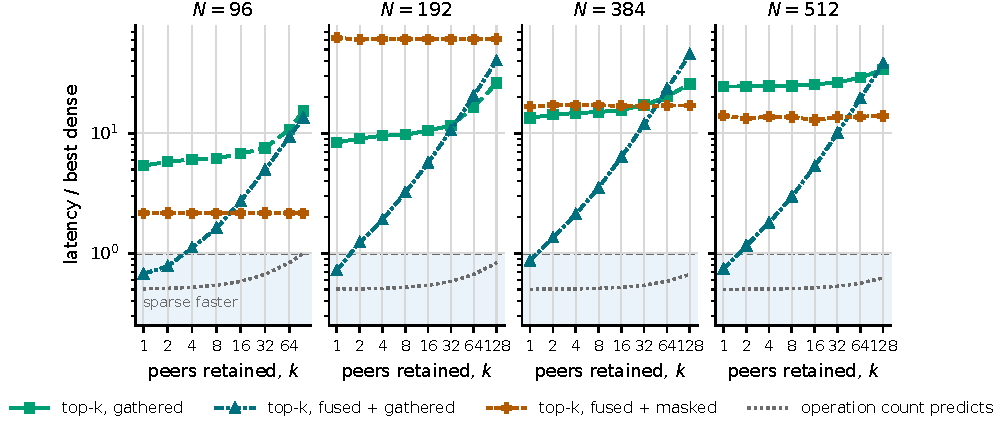
\includegraphics[width=\linewidth]{figures/fig2_ksweep.pdf}
\caption{Latency divided by the faster of the two dense implementations, against
the number of peers retained. The dotted line is what an operation count
predicts for the gathered path, $(N+k)/2N$, which lies below parity everywhere
and so predicts a saving at every sparsity. Shading marks the region in which
sparsity is actually faster; only the fused gathered kernel enters it, and only
at the smallest $k$.}
\label{fig:ksweep}
\end{figure}

\begin{table}[t]
\centering\small
\caption{The sparsity at which a purpose-built sparse kernel stops being faster
than the best dense implementation, and how far it is from parity at the
sparsity multi-agent communication actually uses.}
\label{tab:crossover}
\begin{tabular}{rccrrcrr}
\toprule
& \multicolumn{2}{c}{\textbf{sparsity that pays}} &
  \multicolumn{2}{c}{\textbf{best ratio}} &
  \textbf{replayed, $k{=}1$} &
  \multicolumn{2}{c}{\textbf{at the widest $k$}} \\
\cmidrule(lr){2-3}\cmidrule(lr){4-5}\cmidrule(lr){6-6}\cmidrule(lr){7-8}
$N$ & $k$ & of peers & ratio & at $k$ & min / median & ratio & at $k$ \\
\midrule
192 & $\le 1$ & 0.5\% & 0.76 & 1 & 0.76 / 0.77 & 27.9 & 128 \\
384 & $\le 1$ & 0.3\% & 0.94 & 1 & 0.92 / 0.92 & 18.8 & 128 \\
512 & $\le 1$ & 0.2\% & 0.81 & 1 & 0.77 / 0.77 & 15.4 & 128 \\
\bottomrule
\end{tabular}%

\end{table}

Fusion removes most of the penalty and, at extreme sparsity, reverses the
result. At $512$ agents retaining a single peer, the composed sparse path costs
$4.63$\,ms and the fused one $0.139$\,ms, a factor of $33$ that is attributable
to the implementation and not to the algorithm; the best dense implementation
costs $0.188$\,ms, so the fused sparse path is faster. The manuscript's earlier
claim that no sparse implementation available to us is faster than dense
attention in any measured configuration does not survive, and we report the
correction rather than the claim.

What replaces it is narrower and more useful. A fused sparse kernel is faster
than the best dense implementation only when one or two peers are retained ---
between $0.2\%$ and $2.1\%$ of the available peers, depending on the agent
count --- and the best ratio anywhere in the sweep is $0.66$
(Table~\ref{tab:crossover}). At a quarter of peers, which is the setting the
multi-agent communication literature uses, the best sparse implementation
available to us is $15$ to $26$ times slower than dense attention.

Three things about that crossover matter more than its existence.

The measured advantage stays inside the analytic ceiling. Proposition~\ref{prop:ceiling}
permits at most a twofold reduction in operation count, and the largest speedup
we measure from sparsity, with implementation held constant, is below that. This
is the ceiling behaving as a bound on what is achievable rather than as an
abstraction: once the composed implementation's overheads are removed, the
residual advantage is the one the count allows and no more. It is also why the
first version of these measurements was wrong. Against the library dense path
alone the fused sparse kernel appeared more than twice as fast, which exceeds
what sparsity can supply and was the signal that the baseline, not the
algorithm, was producing the result.

Selection, not aggregation, is what the sparse kernel cannot make cheap. The
argmax-rounds kernel performs $k$ row-wide reductions per query, and reductions
of this shape run at a small fraction of the arithmetic units' throughput
because each is a dependent chain with little instruction-level parallelism.
Its cost is accordingly linear in $k$ and dominates as soon as $k$ exceeds a
handful. The bisection kernel removes that dependence, and the only way it can
is by giving up the compaction --- so the implementation whose selection is cheap
is the one that performs dense aggregation arithmetic. On this hardware a
score-then-select kernel can have sparse arithmetic or $k$-independent
selection, and we could not write one with both.

Fusion is available to dense attention too, and not equally. Dense attention can
stream keys and values in blocks with an online softmax, keeping only a small
tile resident. Exact score-then-select cannot: the complete score row of a query
must exist before the row can be ranked, so the sparse kernel must hold an
$N$-wide tile and its occupancy falls as $N$ grows. That asymmetry is a
consequence of assumption A2 rather than of our implementation, and it is why
the crossover moves to smaller $k$ as the agent count grows.

\subsection{Sensitivity to head width and batch}
\label{sec:sensitivity}

Extending the sweep to head width $512$ resolves a question the earlier version
of this manuscript left open, and resolves it against the direction that version
extrapolated. Reading the ratio down the head-width axis, the crossover exists
only at the two narrowest head widths: the best sparse implementation is faster
than the best dense one at head widths $16$ and $32$ at every agent count, and
at no agent count for head width $128$ or above, where it is roughly twice as
slow (Appendix~\ref{app:grid}). The archival version of this work observed the
ratio falling as head width grew and declined to extrapolate; with the
implementation corrected, the trend runs the other way.

That is what the byte criterion predicts. Byte-neutrality requires
$kd \le N$, so widening the head at fixed agent count tightens the bound on the
retained set proportionally, and at head width $128$ the criterion permits only
$k \le 4$ at $512$ agents --- by which point the selection cost of
Section~\ref{sec:fused} has already overtaken the saving. Widening the batch over a
thirty-twofold range, by contrast, moves the ratio by less than a fifth and
never across parity, which is the expected behaviour of a quantity that is a
ratio of per-element costs.

\subsection{Where the time goes}
\label{sec:stages}

\begin{table}[t]
\centering\small
\caption{Per-stage accounting for both paths at $N{=}\StagesN$. The
last column is the fraction of whichever machine limit binds the stage, and it
separates a stage that is badly implemented from one doing the only thing its
access pattern permits. A figure above $100\%$ marks a stage whose working set
is served from cache, so that its analytic byte count is not traffic to memory;
those stages are the small ones, and none carries an argument.
\StagesCaption}
\label{tab:stages}
\begin{tabular}{lrrrrrrr}
\toprule
\textbf{stage} & GFLOP & GB & FLOP/byte & ms & TFLOP/s & GB/s & \% of limit \\
\midrule
score product & 2.15 & 0.29 & 7.53 & 0.549 & 3.91 & 520 & 35 \\
softmax over $N$ & 0.34 & 0.54 & 0.62 & 0.336 & 1.00 & 1598 & 107 \\
dense aggregation & 2.15 & 0.29 & 7.53 & 0.235 & 9.13 & 1213 & 81 \\
top-$k$ selection & 0.00 & 0.47 & --- & 3.271 & --- & 143 & 10 \\
softmax over $k$ & 0.08 & 0.13 & 0.62 & 0.059 & 1.42 & 2268 & 151 \\
gather of $V$ & 0.00 & 1.21 & --- & 0.954 & --- & 1265 & 84 \\
sparse aggregation & 0.53 & 1.14 & 0.47 & 0.816 & 0.65 & 1398 & 93 \\
\bottomrule
\end{tabular}%

\end{table}

\begin{figure}[t]
\centering
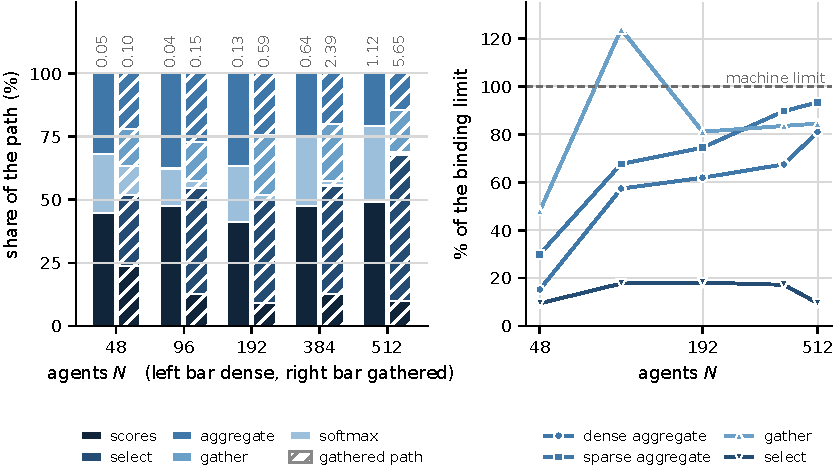
\includegraphics[width=\linewidth]{figures/fig3_stages.pdf}
\caption{\textbf{Left:} how each path divides its time. Selection grows to
dominate the gathered path as the agent count rises. \textbf{Right:} how close
each stage runs to the machine limit that binds it.}
\label{fig:stages}
\end{figure}

Timing each stage in isolation and charging it with its own arithmetic and
traffic corrects an explanation the earlier version of this manuscript offered.
We had attributed the sparse contraction's slowness to a batched
matrix--vector product having lower arithmetic intensity than a real matrix
multiply and being unable to reach the same hardware paths. Measured, that is
wrong. The sparse contraction reaches $93\%$ of the bandwidth the device
attains on a large copy, against $91\%$ for the dense multiply it replaces
(Table~\ref{tab:stages}). Both are bandwidth-saturated and neither is on a
worse hardware path; the sparse one is slower because it moves about four times
the bytes, since the compacted operand carries $kd$ elements per query where the
score row carries $N$. The corrected account is simpler, checkable before the
code is written, and it is the $kd \le N$ criterion of
Section~\ref{sec:composed}.

Selection is a different case, and it is the one stage where the raw
decomposition is misleading in the opposite direction. It is the largest stage
of the composed sparse path, and it runs at under a tenth of the bandwidth the
device attains: it must read the score matrix and write values and indices, and
moving those bytes and nothing else would take a small fraction of the time it
does. That headroom is real, and the fused kernels realise part of it. What no
kernel removes is that the score matrix must be formed and ranked at all, and
the fused measurements of Section~\ref{sec:fused} show what remains once the
headroom is taken.

\subsection{Backward pass and training throughput}
\label{sec:backward}

\begin{table}[t]
\centering\small
\caption{Forward, backward and their sum, for the differentiable
implementations. The sparse path's backward is cheap relative to its forward,
because selection has almost no adjoint, so the gap against fused dense narrows
without closing.}
\label{tab:backward}
\resizebox{\linewidth}{!}{\begin{tabular}{rr rrr rrr rrr rrr r}
\toprule
& & \multicolumn{3}{c}{dense, unfused} & \multicolumn{3}{c}{dense, fused}
& \multicolumn{3}{c}{top-$k$ masked} & \multicolumn{3}{c}{top-$k$ gathered} & \\
\cmidrule(lr){3-5}\cmidrule(lr){6-8}\cmidrule(lr){9-11}\cmidrule(lr){12-14}
$N$ & $k$ & f & b & f+b & f & b & f+b & f & b & f+b & f & b & f+b
& \begin{tabular}[b]{@{}c@{}}gathered f+b\\$\div$ fused f+b\end{tabular} \\
\midrule
192 & 32 & 0.136 & 0.166 & 0.302 & 0.072 & 0.219 & 0.291 & 0.454 & 0.460 & 0.914 & 0.424 & 0.201 & 0.625 & 2.1 \\
384 & 64 & 1.082 & 1.604 & 2.686 & 0.220 & 0.728 & 0.948 & 3.065 & 3.365 & 6.430 & 2.405 & 1.593 & 3.998 & 4.2 \\
512 & 128 & 1.899 & 2.648 & 4.547 & 0.349 & 1.203 & 1.552 & 6.985 & 5.748 & 12.734 & 6.435 & 3.142 & 9.577 & 6.2 \\
\bottomrule
\end{tabular}%
}
\end{table}

Every latency reported so far is a forward pass, which for a training claim is
half the question. Timing forward and backward under the same protocol leaves
the ordering intact and roughly a third of the margin
(Table~\ref{tab:backward}). The gathered path's backward costs about half its
own forward, because the expensive stage --- selection --- has almost no
adjoint: the retained indices are recorded in the forward pass and the backward
is a scatter of gradients into them. Dense attention's backward costs several
times its forward. At $512$ agents the gathered path is $18.5$ times the fused
dense path on the forward alone and $6.3$ times on forward and backward
together; the same narrowing appears at every agent count. The sparse path's
disadvantage in training is therefore substantially smaller than the
forward-only measurements suggest, and remains a disadvantage. The fused kernels are excluded from this comparison: they are
hand-written forward passes, and timing one against an autograd graph would
compare two different things.

\begin{table}[t]
\centering\small
\caption{Where one MAPPO iteration spends its time. Differences between
communication implementations are at or below the iteration-to-iteration spread
in the rightmost column.}
\label{tab:trainstep}
\resizebox{\linewidth}{!}{\begin{tabular}{ll rrrrr rrr}
\toprule
& & \multicolumn{5}{c}{\textbf{share of the iteration (\%)}} & & & \\
\cmidrule(lr){3-7}
$N$ & communication & environment & acting & update fwd & update bwd & optimiser & s/iter & $\div$ fused & spread \\
\midrule
6 & none & 49 & 29 & 11 & 6 & 4 & 2.11 & 1.002 & 4.6 \\
6 & dense, unfused & 48 & 30 & 12 & 6 & 4 & 2.09 & 0.992 & 7.3 \\
6 & dense, library fused & 48 & 30 & 12 & 6 & 4 & 2.10 & 1.000 & 4.0 \\
6 & top-$k$, masked & 48 & 30 & 12 & 6 & 4 & 2.09 & 0.996 & 5.4 \\
6 & top-$k$, gathered & 49 & 29 & 12 & 6 & 4 & 2.13 & 1.011 & 5.3 \\
12 & none & 76 & 14 & 5 & 2 & 2 & 4.35 & 0.998 & 2.3 \\
12 & dense, unfused & 75 & 14 & 6 & 4 & 2 & 4.39 & 1.007 & 3.8 \\
12 & dense, library fused & 75 & 14 & 6 & 3 & 2 & 4.36 & 1.000 & 3.3 \\
12 & top-$k$, masked & 75 & 14 & 6 & 3 & 2 & 4.39 & 1.008 & 5.6 \\
12 & top-$k$, gathered & 75 & 14 & 6 & 4 & 2 & 4.41 & 1.011 & 2.3 \\
24 & none & 92 & 5 & 2 & 1 & 1 & 12.84 & 1.002 & 4.2 \\
24 & dense, unfused & 91 & 5 & 2 & 1 & 1 & 12.98 & 1.013 & 3.3 \\
24 & dense, library fused & 91 & 5 & 2 & 1 & 1 & 12.81 & 1.000 & 1.6 \\
24 & top-$k$, masked & 91 & 5 & 2 & 1 & 1 & 12.80 & 0.999 & 0.8 \\
24 & top-$k$, gathered & 91 & 5 & 2 & 1 & 1 & 12.76 & 0.996 & 1.7 \\
\bottomrule
\end{tabular}%
}
\end{table}

End to end, none of this is visible. Timing a complete training iteration by
phase, with the communication implementation swapped and everything else fixed,
puts the environment at $91\%$ of the iteration at twenty-four agents and
leaves all five implementations within $1.6\%$ of one another, against an
iteration-to-iteration spread of $1.7$ to $3.6\%$ (Table~\ref{tab:trainstep}).
The communication-free variant, which performs no attention at all, is not the
fastest of the five --- which is the clearest available demonstration that this
measurement does not resolve the implementations rather than that it resolves
them as equal. We report it as the null it is. It bounds the practical stakes of
the whole measurement campaign in the regime the training study occupies, and it
is why the computational argument is made on the module in isolation: an effect
a training loop cannot resolve is still an effect, but a paper claiming a
throughput improvement from it would be claiming something it cannot measure.

\subsection{Robustness}
\label{sec:robustness}

The ordering is unchanged under \texttt{torch.compile} and CUDA-graph capture,
at \texttt{bf16}, and on an x86\_64 CPU whose machine balance differs from the
GPU's by more than an order of magnitude. The CPU comparison required
controlling an effect unrelated to attention: with the default allocator the
multi-MiB temporaries each implementation frees between calls are returned to
the kernel and re-faulted on the next call, which at $N{=}192$ adds roughly
$37{,}000$ minor page faults per forward and inflates latency by up to
$8.8\times$. The tax is proportional to the bytes of large temporaries each
implementation churns, so it does not cancel in a ratio, and in an un-pinned run
it inverted the ordering at one configuration. With the heap pinned the
inversion disappears. Appendix~\ref{app:cpu} gives the procedure and both runs.

Because clocks are unlocked and the host is shared, we re-ran the identical
sweep with the device otherwise idle and again under a concurrent load. With the
device idle the ratios reproduce to within a few per cent; under load absolute
latency moves by more than $100\%$ while the paired ratios move by roughly half
that, and every ratio moves against the sparse path. Pairing removes the typical
drift rather than the tail, so the quantity that matters is the margin: no
condition we measured brings a composed sparse implementation below parity, and
the fused crossover reported in Section~\ref{sec:fused} is measured on the
quietest device state we could obtain. Appendix~\ref{app:drift} gives the
figures.


\section{Selecting Before Scoring}
\label{sec:prescore}
Proposition~\ref{prop:escape} says that a selector fixing the retained set
before any score exists is not bound by the twofold ceiling, and that its
operation-count saving grows without limit as the retained set shrinks. That is
a statement about counts, and this paper is about what counts fail to predict.
This section instantiates the escape and measures it.

We use two selectors, both corresponding to mechanisms multi-agent
communication already uses. The first retains each agent's $k$ nearest peers by
Euclidean distance over two-dimensional positions, which is what
neighbourhood-based communication does \citep{jiang2018dgn,jiang2018atoc}. Its
selector is still pairwise, but pairwise in two dimensions rather than in the
head dimension, so it costs a factor of $d/2$ less than forming the scores. The
second orders agents along a Morton curve and retains the $k$ agents adjacent in
that order, at $O(N \log N)$, which satisfies the $o(Nkd)$ condition of
case~(i). Both then evaluate attention scores for the retained pairs only, so
the score term falls from $N^2d$ to $Nkd$ and the ceiling does not apply.

The attention over the retained peers is measured twice: once composed from
library operators, and once as a fused kernel that reads one key row and one
value row per retained peer and accumulates with a running maximum, writing
nothing but the result. Section~\ref{sec:fused} establishes that a composed
constant is an upper bound and not a property of a design, and it would be
incoherent to apply that standard to the mechanism this paper criticises and not
to the one it proposes. The two selectors attend to different peers than a
top-$k$ rule would, so what follows compares cost and not quality, and every
ratio is against the faster of the library dense kernel and our own.

\begin{table}[t]
\centering\small
\caption{Selecting before scoring, at \PrescoreK{} retained peers, every ratio
against the better of the vendor library and our own dense kernel at the tiling
the search of Section~\ref{sec:fused} found. Composing the attention stage from
library operators costs an order of magnitude more than fusing it, and the
difference decides the conclusion: composed, the attention is slower than dense
attention at every configuration measured; fused, it is up to seventeen times
faster.}
\label{tab:prescore}
\resizebox{\linewidth}{!}{\begin{tabular}{rlr rrr r rr}
\toprule
& & \textbf{ops} & \multicolumn{3}{c}{\textbf{measured (ms)}} & \textbf{best}
& \multicolumn{2}{c}{\textbf{$\div$ best dense}} \\
\cmidrule(lr){4-6}\cmidrule(lr){8-9}
$N$ & selector & saved & select & attend & total & dense & attend & total \\
\midrule
48 & nearest neighbours & 8 & 0.151 & 0.064 & 0.167 & 0.035 & 1.85 & 4.85 \\
48 & Z-order window & 10 & 0.367 & 0.059 & 0.386 & 0.035 & 1.72 & 11.18 \\
96 & nearest neighbours & 11 & 0.188 & 0.068 & 0.206 & 0.051 & 1.33 & 4.03 \\
96 & Z-order window & 20 & 0.362 & 0.065 & 0.385 & 0.051 & 1.28 & 7.53 \\
192 & nearest neighbours & 15 & 0.378 & 0.097 & 0.442 & 0.086 & 1.13 & 5.17 \\
192 & Z-order window & 39 & 0.366 & 0.095 & 0.410 & 0.086 & 1.11 & 4.79 \\
384 & nearest neighbours & 17 & 1.871 & 0.173 & 2.024 & 0.169 & 1.02 & 11.96 \\
384 & Z-order window & 78 & 0.374 & 0.171 & 0.478 & 0.169 & 1.01 & 2.82 \\
512 & nearest neighbours & 18 & 4.986 & 0.231 & 5.192 & 0.186 & 1.24 & 27.90 \\
512 & Z-order window & 104 & 0.131 & 0.221 & 0.372 & 0.186 & 1.19 & 2.00 \\
\bottomrule
\end{tabular}%
}
\end{table}

\begin{figure}[t]
\centering
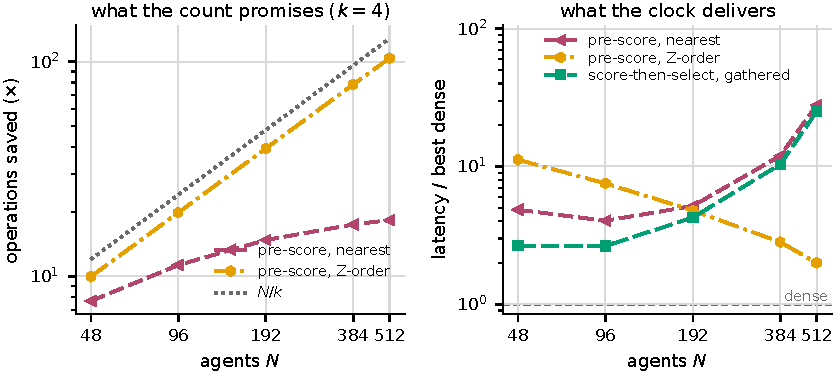
\includegraphics[width=\linewidth]{figures/fig5_prescore.pdf}
\caption{\textbf{Left:} the operation-count saving
Proposition~\ref{prop:escape} promises, which for the sub-quadratic selector
tracks $N/k$. \textbf{Middle:} what the same configurations cost. Fused, the
attention over pre-chosen peers is more than an order of magnitude faster than
dense attention at the largest agent count, and the total is then governed by
the selector, which is where the two selectors diverge. \textbf{Right:} how far
the end-to-end crossing extends. It holds at two and four retained peers, is
level with dense at eight and gone by sixteen.}
\label{fig:prescore}
\end{figure}

Fused, the escape delivers, and how much of it depends on how many peers are
kept. At two retained peers the attention stage costs $0.67$, $0.35$, $0.19$,
$0.08$ and $0.06$ times dense attention from $48$ to $512$ agents; at four,
$0.76$, $0.43$, $0.25$, $0.12$ and $0.09$. The best case over the grid is
$0.060$, nearly seventeen times faster than dense, at $512$ agents and two
retained peers. The advantage narrows as $k$ grows and at sixteen retained peers
it has gone at the smallest agent count, where the stage costs $1.26$ times
dense behind the Z-order selector and $1.58$ behind the nearest-neighbour one,
whose retained rows are scattered rather than adjacent. That shape is what Proposition~\ref{prop:escape} predicts once the score
term shrinks with the aggregation, and no score-then-select implementation
anywhere in this paper comes close to it at any sparsity, because none of them
can remove the score term.

Composed from library operators, the same stage is slower than dense attention
at every one of the forty configurations, by $1.03$ to $6.25$ times. Fusing it
is worth between $3.9$ and $17.4$ times, and the factor grows with the agent
count because the gathered tensor the composition writes and re-reads grows with
it. We report both columns because the composed one is what we measured before
writing the kernel, and on its own it supports the opposite conclusion.

What decides the total is the selector, and the two behave oppositely. The
Z-order selector's cost is nearly flat in the agent count --- $0.096$ to
$0.140$\,ms across the range --- so as attention grows more expensive the
selector's share of the path falls: at four retained peers the whole path costs
$16.8$, $8.8$, $4.0$, $1.28$ and $0.91$ times dense attention from $48$ to $512$
agents. At $512$ agents, selecting before scoring and executing both stages in
kernels written for them is about ten per cent faster end to end than the best
dense attention we can obtain, and the trend is still improving. That crossing
is the whole of it: it holds at two and at four retained peers, the path is
level with dense at eight ($1.01$) and behind it at sixteen ($1.17$), and at
$384$ agents it is behind at every sparsity. Both runs of the sweep put the
crossing cells within one and a half per cent of each other, so the margin is
small but not noise. The nearest-neighbour selector moves the other way. It
materialises an $N \times N$ distance matrix and ranks it --- the same two
operations, on the same shape, that Proposition~\ref{prop:ceiling} says a
score-then-select rule cannot avoid --- so beyond $96$ agents its cost grows
quadratically and the path it belongs to rises to $30.8$ times dense, with the
fused attention stage making no difference to that outcome.

Three things follow, and together they are the paper's constructive result.

Escaping the operation-count ceiling is necessary and not sufficient. Both
selectors escape it, by between $7$ and $107$ times in operations at
four retained peers, and one of
them is an order of magnitude slower than dense attention while the other is
faster. What separates them is whether the selector reaches its decision through
a structure of the size it was introduced to avoid.
Proposition~\ref{prop:escape} charges for the selector in operations, and
operations are the wrong currency: the nearest-neighbour selector's arithmetic
is small and its traffic is exactly the traffic the ceiling is about.

A cheap selector is not sufficient either. With the attention stage composed
from library operators the Z-order path is slower than dense at every agent
count we measure, and only the fused kernel makes the total cross. Both
conditions are needed, and an operation count expresses neither.

And the regime matters. The crossover arrives at a few hundred agents and
improves beyond it, which is above the range most of the multi-agent
communication literature occupies (Section~\ref{sec:related}) and far below the
range where block-sparse attention operates. Whether a method between the two
should sparsify its communication is now a question with a checkable answer
rather than an appeal to an operation count: it depends on whether the selector
avoids a quadratic intermediate, and on whether the sparse attention it leaves
behind is executed in a kernel written for it.


\section{Learning Study}
\label{sec:training}
Sparsification would still be worth having if it cost nothing in return. Testing
that requires care, because on a task where the channel is not needed
``sparsification is free'' and ``the channel was never used'' make identical
predictions. We therefore gate the study on a positive control and register the
analysis plan before the outcomes are inspected. The study is secondary. Its
role is to establish that the architecture being sparsified does something, so
that the sparsification comparisons are not vacuous, and to report what a
five-seed design can and cannot resolve.

\subsection{Design}

Twelve variants at up to twelve agents, five seeds each, two million
environment steps. All scaling in the number of agents is delegated to the
training-free measurements of Section~\ref{sec:measurement}, because an
end-to-end training step in this pipeline is dominated by the environment
(Section~\ref{sec:backward}) and cannot attribute a latency difference to the
communication module.

Two positive controls establish that the channel carries something. The first is
a reference task in which each agent observes only its partner's goal, so
information must pass between agents; it is fixed at two agents, where the
selection mechanism is degenerate, so it validates the message pathway rather
than the selection. The second is a partially observable variant of a standard
cooperative task, introduced here, in which a peer's relative position is
withheld beyond a fixed radius. Under a uniform random policy the fraction of
peers visible falls with the number of agents while the absolute number visible
rises, because the world does not grow: that is a difficulty confound across
agent counts, and it is why no claim in this paper compares returns across agent
counts in this environment.

The analysis plan was committed after eight of the forty runs in the
pre-registered family had completed and before any of their outcomes was
inspected; the two positive controls were complete and had been inspected, which
is why they are excluded from the inferential family.
Appendix~\ref{app:prereg} gives the chronology and the single amendment. The
plan fixes the endpoint, the six comparisons and their direction, an exact
two-sided permutation test, the effect sizes, a percentile bootstrap interval
flagged approximate at five seeds, and a Holm--Bonferroni correction. It also
fixes the power expectation in advance: with five seeds per variant the smallest
attainable two-sided $p$-value is $2/252 = 0.0079$ against a first Holm
threshold of $0.05/6 = 0.0083$, a margin of $4\times10^{-4}$, so a first
rejection requires one variant's five seeds to lie entirely above the other's.
Any null in this family is under-powered rather than evidence of absence, and no
equivalence claim is available because no equivalence margin was registered.

\subsection{Results}

\begin{table}[t]
\centering\small
\caption{The two positive controls, which were inspected before registration and
are excluded from the correction, and the primary pre-registered comparison.
$A-B$ is the difference of means and $d$ the standardised effect.
Appendix~\ref{app:training} gives the remaining five comparisons.}
\label{tab:training}
\begin{tabular}{lrrrr}
\toprule
& $A-B$ & 95\% interval & $d$ & $p$ \\
\midrule
\multicolumn{5}{l}{\emph{Positive controls, descriptive}} \\
communicating $-$ non-communicating, reference task
  & $+4.26$ & $[+3.15, +5.23]$ & --- & $0.0079$ \\
communicating $-$ non-communicating, partially observable
  & $+11.59$ & $[+7.13, +16.44]$ & --- & $0.0079$ \\
\midrule
\multicolumn{5}{l}{\emph{Primary pre-registered comparison}} \\
attention-selected peers $-$ uniformly random peers, same budget
  & $+4.03$ & $[-3.35, +11.42]$ & $+0.60$ & $0.357$ \\
\bottomrule
\end{tabular}
\end{table}

Both positive controls separate completely, each attaining the floor of the
permutation test for this design (Table~\ref{tab:training}). Measured attention
entropy on the partially observable control is $0.35$ nats against a ceiling of
$1.61$, so the learned weighting is peaked rather than uniform. What this
establishes is that sparsification is being applied to an architecture whose
communication machinery improves return under the evaluated setup. It does not
establish that the learned attention channel alone accounts for the difference:
the communicating variants carry $7$--$19\%$ more trainable parameters, and the
reference task supplies a discrete utterance channel of its own. A
parameter-matched sham-communication variant would be needed for the
channel-specific causal claim, and we do not make it.

The comparison the design exists for holds the communication budget, the
executed aggregation cost and every hyperparameter fixed, and varies only
whether peers are chosen by attention score or uniformly at random. Its point
estimate favours attention by roughly two thirds of a standard deviation and its
interval includes zero. The design lacked the power to resolve an effect of that
size, which the pre-registered power calculation said in advance; nothing
follows about whether attention selects informatively. The remaining five
comparisons are reported in Appendix~\ref{app:training} as point estimates with
intervals \citep{agarwal2021rliable}, and all six are Holm-adjusted nulls. No
conclusion in this paper rests on any of them.

Two limits of the environment bound what the study can say. At twelve agents
neither variant learns the task well: the dense variant scores below a
uniform-random policy and the sparse variant only just above it, so no
comparison at that agent count is interpretable. And the centralised critic sees
the same masked observations as the actors rather than a privileged global
state, which departs from standard practice for this learner and is a plausible
contributor to that failure.


\section{Sources of Measurement Error}
\label{sec:pitfalls}
Each error described below produced a spurious result during this study before
it was caught, and in each case the first symptom was a plausible number rather
than an obvious error. The causes
group into four kinds, and the grouping is useful because the kinds differ in
how they are caught. Table~\ref{tab:pitfalls} lists them with the corrective
practice each forced.

\paragraph{Instrumentation.} A diagnostic that synchronises the device inside
the timed region measures the synchronisation. Our attention module computed an
entropy statistic through a call that transfers a scalar to the host, and with
it enabled dense latency was nearly flat in $N$ while its work grew by two
orders of magnitude --- a result we briefly read as evidence that the quadratic
cost does not manifest. Synchronising without naming the device is the
complementary error: work submitted to a non-default device is never waited on,
and every kernel at every size then reports the event-resolution floor of about
$0.4\,\mu$s. On the host, the default allocator returns the multi-MiB score
matrices each implementation frees between calls, so the next call re-faults
them; at $N{=}192$ that added roughly $37{,}000$ minor page faults per forward
and inflated latency by up to $8.8\times$. Errors of this kind leave traces ---
an impossible latency, a curve that is flat where it should be quadratic, a
non-monotone cost --- and are caught by looking at the shape of the result
rather
than its value.

\paragraph{Interference from a shared device.} Timing implementations in
sequential blocks makes each block hostage to whatever else was running during
it. On our shared host the recorded inter-run spread reaches $374\%$ at one
configuration of the released sweeps, and the sessions that produced our tiling
searches differ from each other by up to $81\%$ on identical shapes. Interleaving the implementations repetition by repetition lands any
interference burst on all of them at once, so the ratios between them survive
even when the absolute numbers drift. The residual sensitivity is to which
implementations share an interleaved sweep: at small $N$, where a fixed per-call cost is a large share of the
measurement, the launch count of the whole group enters every measurement in it,
and two of our own sweeps that differ only in which implementations they time
disagree by $1.4\times$ at twelve agents. Sweeps that will be compared
must therefore hold their implementation set fixed and say so.

\paragraph{Measuring a different algorithm from the one claimed.} The two most
dangerous errors are of this kind, because the resulting numbers are internally
consistent, reproducible, and stable under every check the others would fail.
They answer a different question from the one being asked. Applying top-$k$ as a
mask leaves the dense aggregation matmul in place, so the advertised saving is
never executed; a FLOP model based on $1-k/(N-1)$ nonetheless credits that code
with a $75\%$ saving at $N{=}512, k{=}127$, and with more than $90\%$ wherever
$k/(N-1) < 0.1$. Comparing against unfused dense alone is the same error in the
baseline: at $N{=}512$ the unfused and fused dense paths differ by $5.4\times$,
so which one is meant sometimes changes the answer. The defence is to state the
operation count each implementation executes alongside its latency, and to check
which backend actually serves each shape and dtype, both of which make a
mismatch between the claimed and the executed algorithm visible immediately.

\paragraph{Attributing implementation quality to the algorithm.} The fourth kind
appeared only when we wrote our own kernels. Timing a hand-written sparse kernel
against a vendor library's dense kernel measures sparsity and authorship at
once. At the head widths used in multi-agent communication, PyTorch's fused
attention path runs at roughly half the rate of a straightforward Triton kernel,
because it is tuned for the long sequences and wide heads of language models.
Against it our fused sparse kernel appears up to $2.8\times$ faster, which is
more than sparsity can supply at any $k$ and was how we noticed. Matched
authorship is the obvious remedy and it is not sufficient either: two kernels by
the same author can differ by more than the margin under test. The condition
that identifies the algorithm is matched \emph{efficiency}, so we search one
parameter space for both under one admissibility filter --- which admits very
unequal numbers of configurations, and we report those counts too --- and give
the fraction of the device's own arithmetic rate each kernel reaches
(Section~\ref{sec:fused}). That is also what
reveals when neither implementation is near the machine, which is a different
warning and one worth having: a comparison between two kernels at a third of
peak resolves the algorithms only if the margin exceeds the headroom, and ours
does not everywhere.

\begin{table}[t]
\centering
\small
\caption{Eight ways a benchmark measures something other than the algorithm,
each of which produced a spurious result in this study. The first five are
caught by the shape of the result; the last three are not, because the numbers
they produce are self-consistent.}
\label{tab:pitfalls}
\begin{tabular}{p{0.12\linewidth}p{0.26\linewidth}p{0.24\linewidth}p{0.26\linewidth}}
\toprule
\textbf{Kind} & \textbf{Cause} & \textbf{Symptom} & \textbf{Corrective practice} \\
\midrule
\multirow{3}{*}{\parbox{\linewidth}{Instrumen\-tation}}
& Host transfer inside the timed region &
Dense latency nearly flat in $N$ &
Gate diagnostics behind a flag that is off while timing \\
\addlinespace
& Synchronisation without a device argument &
Every kernel reports the event-resolution floor &
Pin the device and pass it to every synchronisation \\
\addlinespace
& Host allocator returning large temporaries &
Up to $8.8\times$ inflation and a non-monotone curve &
Pin the heap; count minor faults per forward \\
\midrule
\multirow{2}{*}{Interference}
& Timing implementations in sequential blocks &
Swings above $100\%$ between identical configurations &
Interleave repetition by repetition; report paired ratios \\
\addlinespace
& Changing which implementations share a sweep &
Two sweeps disagree by $1.4\times$ at twelve agents &
Fix the implementation set across comparable sweeps \\
\midrule
\multirow{2}{*}{\parbox{\linewidth}{Wrong algorithm}}
& Benchmarking a masked implementation as sparse &
The advertised saving is never executed &
Assert executed FLOPs differ and trace the products issued \\
\addlinespace
& Comparing only against unfused dense &
A $5.4\times$ more favourable comparison at $N{=}512$ &
Report both baselines; check which backend serves the shape \\
\midrule
\parbox{\linewidth}{Wrong\\ baseline}
& A hand-written sparse kernel against a vendor's dense kernel &
An apparent speedup larger than the analytic ceiling permits &
Write the dense baseline in the same framework and tiling \\
\bottomrule
\end{tabular}
\end{table}

One belief of our own also needed correcting. We assumed that standard counters
are blind to fused attention kernels, which would make a FLOPs-only comparison
unable to see the baseline that matters. In PyTorch 2.11 that is not so:
\texttt{torch.utils.flop\_counter} reports the fused path correctly, and it was
our harness that added an analytic term on top of the counter's output for that
implementation, publishing a figure $1.83\times$ too large. The narrower point
generalises better than the one we started with: a counter has to be validated
against the kernels it is expected to observe, because only a counter attached
to the running program can contradict a FLOP model.


\section{Limitations}
\label{sec:limitations}
\paragraph{Measurement error.} Seven errors produced plausible but spurious
results during this study before they were caught, among them a host transfer
inside the timed region, sequential timing on a shared device, a masked
implementation benchmarked as sparse, and a hand-written sparse kernel compared
with a vendor dense kernel tuned for another regime. Appendix~\ref{sec:pitfalls}
lists each with its symptom and the practice that corrected it.

\paragraph{Limitations.} Every cost result concerns centralised inference on a
single device; the paper makes no claim about bandwidth-constrained distributed
deployment, where reducing transmitted messages is itself the objective and
top-$k$ selection may well be the right design. The analysis is single-round
and single-head. The operation-count ratio is invariant to rounds and heads, but
the timing result is not guaranteed to be: $H$ heads of width $d/H$ change the
per-head width, which is the axis along which our timing result changes sign.

The measured envelope is one GPU architecture (NVIDIA Blackwell, sm\_120), one
x86\_64 CPU, PyTorch 2.11 with CUDA 12.8 and Triton 3.6, head widths $16$ to
$512$, $N \le 512$, batch $32$ to $1024$, and fp32, TF32 and bf16. We could not replicate on a second
GPU generation, because no other was available to us. Both cards were shared
with other tenants throughout, and clocks could not be locked; every claim is
therefore a ratio between implementations timed in the same interleaved sweep,
and no claim is read off an agent count below $192$, where a fixed per-call cost
is a large share of the measurement.

Our kernels are not optimal. The sparse kernels hold the whole score row of a
query on chip, which caps them at $N \le 1024$ and admits only three tilings
above $192$ agents against $28$ to $106$ for the dense kernel; a streaming exact
top-$k$ that keeps a running candidate set would not have that constraint, and
we did not write one. The sparse efficiency figures are therefore lower bounds,
and the negative results at wide heads are weakly supported. The fused
crossover at one retained peer is provisional in the other direction, and
Section~\ref{sec:precision} shows how: a dense kernel that uses the tensor cores
removes it from $384$ agents upward. The
pre-score selectors attend to a different peer set than top-$k$ does, so their
comparison is of cost and not of quality; their selectors are composed from
library operators, so the selector costs we report are upper bounds; and their
envelope is one head width, one batch and fp32. Finally, the learning study
(Appendix~\ref{sec:training}) has five seeds per variant; it shows that the
communication architecture improves return and cannot resolve the effect of any
sparsification choice.


\section{Conclusion}
\label{sec:conclusion}
We asked when an operation-count saving from sparse attention in multi-agent
communication becomes a saving in time, and answered by charging every
peer-selection rule for the cost of deciding. A rule that ranks scores must form
all of them, so at most half of the forward-pass multiply--accumulates are
removable; composed from library operators it is slower than dense attention
everywhere we measure, and fused it pays only at one or two retained peers,
because finding the retained set takes most of its time. Selecting before
scoring is where the saving can become real, and the selector then decides the
outcome. At the agent counts multi-agent methods use, the number of kernels a
step launches decides latency before either. A speedup claimed for sparse
communication therefore has to be measured, on the kernel that runs and against
the strongest dense baseline for the format.


\subsubsection*{Broader Impact Statement}
This work is a measurement and correction study of a computational-efficiency
claim. It introduces no new capability and no new data. Its intended effect is
to reduce wasted compute in the design of multi-agent communication
architectures by discouraging optimisation against an operation count that does
not predict runtime.

\bibliographystyle{tmlr}
\bibliography{references}

\appendix
\section{Additional benchmark results}
\label{app:grid}

\subsection{The full parameter grid}

Table~\ref{tab:grid} gives the best-over-implementations sparse latency divided
by the best-over-implementations dense latency, across head width and across
batch, at each agent count and at the most favourable sparsity available. Head
width is swept to $512$ and batch from $32$ to $1024$. The largest batch we
attempted, $4096$ at $512$ agents, could not be measured: the score matrix alone
runs to several gigabytes and the device is shared, so that configuration is
absent.

\begin{table}[ht]
\centering\small
\caption{Best sparse divided by best dense, over head width (upper block) and
batch (lower block). Values below one would indicate sparsity winning.}
\label{tab:grid}
\begin{tabular}{rrrr}
\toprule
head width $d$ & $N{=}96$ & $N{=}192$ & $N{=}512$ \\
\midrule
16 & 0.66 & 0.71 & 0.74 \\
32 & 0.51 & 0.69 & 0.62 \\
64 & 0.87 & 1.32 & 2.15 \\
128 & 1.38 & 2.17 & 1.88 \\
256 & 2.10 & 2.07 & 2.11 \\
512 & 1.66 & 1.72 & 2.18 \\
\bottomrule
\end{tabular}

\vspace{1em}

\begin{tabular}{rrrr}
\toprule
batch $B$ & $N{=}96$ & $N{=}192$ & $N{=}512$ \\
\midrule
32 & 0.55 & 0.65 & 0.57 \\
1024 & 0.55 & 0.75 & 0.72 \\
\bottomrule
\end{tabular}%

\end{table}

\subsection{Dispersion behind the headline numbers}
\label{app:dispersion}

The primary statistic is the minimum over interleaved samples, on the modelling
assumption that contention can only add time. That statistic is trustworthy only
if the underlying sample was not wildly dispersed, so the harness records the
median, the interquartile range and the spread of per-run medians for every
configuration, and the released artifacts carry all of them. Two properties of
this host limit what any of it can mean. Both GPUs carried between 30 and
80~GiB
of other tenants' allocations and near-continuous utilisation throughout the
campaign, and clocks could not be locked. We therefore report the spread of
per-run medians beside every configuration rather than a confidence interval: a
ratio of minima has no sampling distribution.

\subsection{Drift control}
\label{app:drift}

The headline sweep was repeated in full on the same device, hours later and
under different load from other tenants. Table~\ref{tab:drift} gives how far
each agent count moved between the two runs, in absolute latency and in the
ratio against the best dense implementation, which is the quantity every claim
is stated in.

\begin{table}[ht]
\centering\small
\caption{Movement between two runs of the identical sweep. From $192$ agents
upward both the latencies and the ratios reproduce to about one per cent. At
$96$ they do not, by a wide margin, which is why no claim in this paper is read
off an agent count below $192$.}
\label{tab:drift}
\begin{tabular}{rrrrrr}
\toprule
& & \multicolumn{2}{c}{\textbf{latency} $|\Delta|$ (\%)}
& \multicolumn{2}{c}{\textbf{ratio} $|\Delta|$ (\%)} \\
\cmidrule(lr){3-4}\cmidrule(lr){5-6}
$N$ & configurations & median & max & median & max \\
\midrule
96 & 44 & 0.1 & 4.2 & 0.3 & 2.5 \\
192 & 44 & 0.2 & 6.1 & 0.2 & 6.0 \\
384 & 44 & 0.7 & 11.3 & 0.5 & 11.6 \\
512 & 44 & 6.1 & 12.0 & 7.2 & 12.6 \\
\bottomrule
\end{tabular}%

\end{table}

From $192$ agents upward the measurement is stable: median movement is under
one per cent in latency and under half a per cent in the ratio, with the worst
single configuration under eleven per cent. At $96$ agents it is not stable at
all --- every implementation ran between $14\%$ and $394\%$ slower in the second
run, and the fastest configurations in the first run had recorded inter-run
spreads above $85\%$ at the time. That is the signature of a launch-bound
regime on a contended device rather than of anything about attention, and it is
why the crossover of Section~\ref{sec:fused} is reported only from $192$ agents
upward even though the sweep measures smaller ones.

The repeat is on the same physical card, so it establishes stability across
runs and hours, not independence from one device, and we were not able to
obtain a second card free of other tenants. It covers the sweep of
Section~\ref{sec:composed} and Section~\ref{sec:fused}'s figure; the tiling
search of Table~\ref{tab:autotune} was run once, so the crossover it reports
carries the reproducibility of a single session rather than of a repeat.
Measurements were taken on both cards of this host --- the core sweeps, the
search and the stage accounting on one, the head-width sweep and the
pre-score measurements on the other --- and no cross-device calibration is
claimed, which is a further reason no figure from one is divided by a figure
from the other.

\section{Implementation and measurement validation}
\label{app:verification}

\subsection{Functional equivalence}

Every implementation is checked against the reference at every configuration
whose latency any released artifact reports: $158$ combinations of agent count,
head width and retained-peer count, $136$ of them with $k < N-1$ so that
selection is actually exercised, over $1.25$ million query rows in total. The
check matters more than it looks. Exact top-$k$ is discontinuous in the scores,
so two implementations that accumulate the score product in different orders can
rank a near-tied pair differently and aggregate over different peers, producing
a large output difference from a rounding-level score difference. An earlier
version of our per-query fused kernel computed the score row as a reduction
instead of through the matrix-multiply units and disagreed with the reference at
a handful of configurations for exactly that reason; the kernels reported here
use the same product as the reference.

With that fixed, every implementation agrees with the reference to
\texttt{fp32} rounding --- maximum deviation $3.2\times10^{-6}$, and zero for
the two implementations that share the reference's operator sequence exactly ---
with one attributable exception. The fused kernel that selects by threshold
retains every peer at or above the $k$-th largest score, so an exact tie at that
boundary retains $k{+}1$ peers where a rank-based selection retains $k$. Four
query rows in $1.25$ million have such a tie, at three of the $158$
configurations, and those four rows are the only place any implementation
differs from the reference by more than rounding. The check is run by
\texttt{scripts/verify\_all\_configurations.py}, which classifies a tie
divergence separately from a failure so that the distinction is in the artifact
and not only in this paragraph.

\subsection{What each implementation executes}

The masked and gathered implementations compute the same function while
executing different work, which is the distinction the paper turns on, so
regression tests pin it. Maximum absolute deviation
between the two paths is below $10^{-10}$ in \texttt{float64}. A FLOP counter
attached to the running program reports identical totals for dense and masked
--- the counter scores matrix products, and masked issues the same two as dense
--- against a smaller total for gathered, the difference being exactly the
aggregation term. Tracing every matrix product confirms that the gathered path
issues no dense aggregation product and does issue the compacted one, and that
every top-$k$ variant still issues the full score product, which is assumption
A2 made mechanical.

\subsection{Which backend serves the fused dense baseline}

A probe forces each scaled-dot-product backend in turn, at both dtypes and at
three agent counts, under no mask, an additive float mask and a Boolean mask,
and the profiler records which kernel the default dispatcher launches. The
FlashAttention backend is rejected under any non-null mask in either form, and
in \texttt{fp32} under any input, so the library dense baseline runs the
memory-efficient CUTLASS kernel. Forcing FlashAttention on the same unmasked
\texttt{bf16} shape is faster than the kernel we do get, so a baseline able to
reach it would widen rather than narrow the gap we report --- which is part of
why the dense baseline in this revision is the better of the library path and a
kernel we wrote.

\subsection{The host allocator control}
\label{app:cpu}

Dense, masked and gathered each allocate and free several multi-MiB score
matrices per forward. The default allocator returns those pages to the kernel
and they are re-faulted on the next call, which at $N{=}192$ adds roughly
$37{,}000$ minor page faults per forward and inflates latency by up to
$8.8\times$. The tax is proportional to the bytes of large temporaries each
implementation churns, so it differs per implementation and does not cancel in a
ratio; in an un-pinned run it inverted the ordering at one configuration. We
raise the allocator's retention threshold so that freed temporaries are kept,
and count minor faults per forward from the process's own resource usage across
the timed region. The harness records the allocator environment, the thread
counts, the affinity mask and the fault totals in each run's metadata, and the
superseded un-pinned run is retained beside the pinned one.

\subsection{Machine balance}
\label{app:roofline}

Peak arithmetic rate is measured with a large matrix multiply and peak bandwidth
with a large copy, in the same process as the measurements they normalise. That
matters here more than it usually would: on this shared host the peak we measure
varies between $53$ and $77$~TFLOP/s across sessions, depending on what else is
running. Every fraction-of-peak figure in the paper is against the peak measured
in the same process as the number it normalises, and is therefore an upper bound
on the true efficiency rather than an estimate of it. Comparisons between two
implementations measured in one process are unaffected; comparisons of a
fraction across sections are not, and we make none. The
copy source is written before it is read: an untouched allocation on this
operating system is backed by the shared zero page, so a host-side copy from it
re-reads one cache line and reports a bandwidth several times the machine's
real figure, and an earlier version of this probe did exactly that: every CPU
ridge point derived from it was too large by roughly a factor of six. Device
work is also timed with device events rather than host wall-clock, since host
timing around a sub-millisecond copy measures launch and synchronisation. The
probe reports two ridge points per device, one with a cache-resident buffer and
one with a buffer larger than the last-level cache, because the two differ by a
factor of two on the host and a claim that holds for one need not hold for the
other.

\section{Additional training analysis}
\label{app:training}

\subsection{Pre-registration chronology}
\label{app:prereg}

The analysis plan was committed when eight of the forty runs in the
pre-registered family had produced a final evaluation and before any of their
returns had been inspected. Commit history establishes the ordering: the
positive-control artifacts at 12:18, the plan at 12:56, and the remaining
artifacts at 19:11 the same day. The plan has two commits, the second appending
to its deviations log; the endpoint, comparisons, test, effect sizes, interval
and correction are byte-identical to the pre-unblinding version. Timestamps
establish ordering and nothing more. Data generation had demonstrably already
begun.

One correction is logged against the released plan. It asserts that at most one
comparison in the family can reach corrected significance. That is false: Holm
is a step-down procedure, so once a first rejection is obtained its later
thresholds are looser and further rejections remain possible. The manuscript
states the corrected version; the deviation is logged against the released plan.

\subsection{The remaining comparisons}

Five further comparisons were registered and all are Holm-adjusted nulls. Two
deserve a note. The comparison at twelve agents has the one sign opposite to
its registered direction and carries the family's largest point estimate, and
we set it aside on the ground that neither variant learns the task there. That
ground was not registered: it is a post-hoc exclusion of the largest observed
effect, we have logged it as a deviation against the released plan, and a
reader who rejects it should read the comparison as an under-powered null with
a large point estimate, which is what the registered analysis returns either
way. The evidence for the exclusion is this. A uniform-random policy scores
$-758.9$ under a forty-episode evaluation,
against $-864.9$ for the dense variant, which is worse, and $-717.9$ for the
sparse variant, which is better but barely learning; the comparison is between a
diverged run and a struggling one. Separately, for two comparisons the bootstrap
interval excludes zero while the permutation test does not. The registration
named the permutation test, so it governs; the disagreement is unsurprising at
five seeds, where the interval is coarse, discrete and of uncertain coverage. We
report both so that the estimated effect and the strength of evidence for it are
both visible.

Descriptively, and supporting no claim: the budgeted variant meets its budget
but not by the intended route, its gate collapsing to an expected support near
one within the first tenth of training while the dual multiplier decays to zero;
the entmax variant settles at a support of $1.64$ of five peers; and attention
entropy falls from $0.35$ nats over five peers to $0.12$ over two. The three sit
on different supports and are reported only as an instrumentation check.

\subsection{The partially observable environment}
\label{app:env}

The variant modifies the standard cooperative task in one respect: a peer's
relative-position entry is zeroed when the peer is farther than a fixed radius.
Reward, action space, landmark observations, episode length and observation
dimension are unchanged. Two properties limit what it can support. The mask is a
zeroing rather than an explicit visibility flag, so a peer at relative position
exactly zero is not distinguishable from an absent one; measured under a uniform
random policy, this affects at most $0.15\%$ of visible peers. And the visible
fraction falls with the number of agents while the absolute number visible
rises, because the world size is fixed, which is a difficulty confound that
rules out across-agent-count return comparisons.

The communicating variants carry between $7.2\%$ and $19.0\%$ more trainable
parameters than the communication-free baseline, since the attention module adds
parameters the baseline has no analogue for. The positive controls therefore
establish that the communicating architecture outperforms the baseline, not that
the channel alone accounts for the difference.

\section{Literature audit}
\label{app:audit}

For each audited paper we read the full text, including appendices and the
official supplement where one exists --- through the ar5iv rendering of the
arXiv version where the paper is on arXiv, and the venue's own copy
otherwise --- searched it for seven temporal keywords,
and recorded whether it makes a computational-efficiency or complexity claim
about its mechanism, whether it reports any measured temporal quantity
attributable to that mechanism, and the figure, table or sentence that settled
the decision. A statement such as ``training took a few days'' does not qualify,
since it is not attributable to the mechanism. Scope matters for at least one
entry, whose affirmative verdict rests on a wall-clock figure in an appendix and
would be negative on the main body alone. This is an audit of reporting practice
in a small, deliberately selected set --- the papers we ourselves relied on ---
and not a sample of either literature; a negative verdict means the argument
rests on operation counts or asymptotics, not that it is wrong.

\begin{table}[ht]
\centering\small
\caption{The twelve audited papers, their efficiency claim, the kind of evidence
it rests on, and whether any measured temporal quantity attributable to the
mechanism appears anywhere in the paper or its supplement. A ``no'' means the
argument rests on operation counts or asymptotics, not that it is wrong.}
\label{tab:audit}
\begin{tabular}{p{0.29\linewidth}p{0.36\linewidth}p{0.14\linewidth}l}
\toprule
\textbf{Paper} & \textbf{Efficiency claim} & \textbf{Type} &
\begin{tabular}[b]{@{}l@{}}\textbf{Measured}\\\textbf{time?}\end{tabular} \\
\midrule
\multicolumn{4}{l}{\emph{Multi-agent communication and attention}} \\
\citet{das2019tarmac} & Qualitative bandwidth argument only & qualitative & no \\
\citet{jiang2018atoc} & Communication is 'restricted by bandwidth\,\ldots & agent/message counts & no \\
\citet{jiang2018dgn} & receiving a large amount of information\,\ldots & asymptotic / qualitative & no \\
\citet{singh2018ic3net} & continuous communication allows efficient\,\ldots & message counts / convergence epochs & no \\
\citet{sukhbaatar2016commnet} & none explicit & --- & n/a \\
\citet{wen2022mat} & Sequence modelling 'reduces the complexity\,\ldots & asymptotic & \textbf{yes} \\
\multicolumn{4}{l}{\emph{Efficient attention and sparse mixture-of-experts}} \\
\citet{beltagy2020longformer} & Sliding-window + global attention scales\,\ldots & asymptotic & \textbf{yes} \\
\citet{choromanski2021performers} & FAVOR+ gives linear rather than quadratic\,\ldots & asymptotic & \textbf{yes} \\
\citet{fedus2022switch} & Sparse routing increases parameters at\,\ldots & FLOPs-matched & \textbf{yes} \\
\citet{kitaev2020reformer} & LSH attention reduces O(L$2$) to O(L log L) & asymptotic & \textbf{yes} \\
\citet{shazeer2017moe} & 1000x capacity increase at minor\,\ldots & FLOPs + measured & \textbf{yes} \\
\citet{zaheer2020bigbird} & reduces this quadratic dependency to linear';\,\ldots & asymptotic + memory & no \\
\bottomrule
\end{tabular}%

\end{table}

\section{Reproduction and provenance}
\label{app:repro}

The measurement campaign is training-free and completes in under an hour on one
device. \texttt{scripts/run\_revision\_campaign.sh} regenerates every artifact
in the order the manuscript reports them;
\texttt{scripts/make\_revision\_tables.py} and
\texttt{scripts/make\_revision\_figures.py} regenerate every table and figure
from those artifacts, so no tabular number in the manuscript is transcribed by
hand; and \texttt{scripts/check\_revision\_numbers.py} re-derives the numbers
that appear in prose and fails on any disagreement.

Three provenance caveats. The hardware description and the aggregate provenance
record were written before this project's environment was upgraded and describe
a superseded software stack and a host that is no longer available; both have
been corrected, and the run-level provenance for the training variants lives in
the per-run configuration files rather than in the aggregate record. The GPUs
used for every measurement in this paper are shared with other tenants, so
absolute latencies are not reproducible to better than the drift reported in
Appendix~\ref{app:drift} and only ratios between implementations timed in the
same interleaved sweep should be compared. And the activation-memory measurement
is reported from a run with the card otherwise free, since a shared-host repeat
exhausts memory one agent count earlier.


\end{document}
